\appendix
\section{Attention: from similarity scores to a weighted output}\label{app:attention}
\subsection{The operation and its dimensions}
For one attention head, let $X\in\mathbb{R}^{n\times d_{\mathrm{model}}}$ contain $n$ token or image-patch representations, one per row. The notation $\mathbb{R}^{n\times d}$ means a matrix of real numbers with $n$ rows and $d$ columns; $d_{\mathrm{model}}$ is the number of features per representation. Learned projection matrices give $Q=XW_Q$, $K=XW_K$, and $V=XW_V$, with $Q,K\in\mathbb{R}^{n\times d_k}$ and $V\in\mathbb{R}^{n\times d_v}$. Thus $d_k$ is the query/key dimension and $d_v$ the value dimension. A superscript $\top$ denotes transpose, exchanging rows and columns. Scaled dot-product attention is
\begin{equation}\label{eq:attention}
 A=\operatorname{softmax}_{\mathrm{row}}\!\left(\frac{QK^\top}{\sqrt{d_k}}+M\right),
 \qquad Z=AV.
\end{equation}
The $n\times n$ matrix $A$ contains normalized weights; $Z$ has shape $n\times d_v$. For scores $s_{ij}$, row-wise softmax computes $A_{ij}=e^{s_{ij}}/\sum_\ell e^{s_{i\ell}}$: exponentiate each score and divide by the total in its row. An optional mask $M$ excludes disallowed positions by adding $-\infty$ to their scores, making their exponential zero; allowed positions receive zero in $M$. With finite allowed scores and at least one allowed key, each row of $A$ sums to one. Causal masking prevents access to later positions when predicting a sequence one token at a time. In cross-attention, queries and keys/values come from different sequences and $A$ need not be square \citep{vaswani2017}.

\subsection{An original two-key calculation}
Take one query $q=(1,0)$, two keys $k_1=(1,0)$ and $k_2=(0,1)$, and scalar values $v_1=2$, $v_2=10$. With $d_k=2$ and no mask, the scores are $z_1=1/\sqrt{2}$ and $z_2=0$. Thus
\begin{align}
\alpha_1&=\frac{e^{1/\sqrt{2}}}{e^{1/\sqrt{2}}+1}\approx0.6698,
&\alpha_2&\approx0.3302,\\
o&=\alpha_1\,2+\alpha_2\,10\approx4.6419.
\end{align}
The larger match receives more weight, but the other value still contributes. If both scores were equal, the output would be their average, 6. If only the first key were allowed by the mask, the output would be 2. These are consequences of this toy calculation, not measurements from a trained model.

The weights alone do not determine the output. Keeping the same query and keys while changing $v_2$ from 10 to $-10$ leaves the displayed attention weights unchanged, yet changes the output from about 4.6419 to $-1.9629$. This is a simple counterexample to treating a weighting plot as a complete explanation of the computation. The example is reproduced in \texttt{code/src/brainsmodels/clinical\_appendix.py}.

To check the intermediate arithmetic, $e^{1/\sqrt{2}}\approx2.0281$, so the weights are approximately $2.0281/3.0281$ and $1/3.0281$. Using the unrounded weights, their contributions to the original output are $\alpha_1v_1\approx1.3395$ and $\alpha_2v_2\approx3.3024$. The second value contributes more despite its smaller weight. In the intervention, only the sign of that second contribution changes. \coursenotebook{10_two_key_attention.ipynb}{Notebook 10} performs the calculation at full precision.

Why divide by $\sqrt{d_k}$? Under the illustrative assumptions that query and key components are independent, zero-mean, and unit-variance, their dot product has variance $d_k$. Scaling gives variance one. Large unscaled scores can concentrate softmax weights and reduce its local sensitivity. This calculation motivates the scale; it does not assert that trained representations meet those distributional assumptions exactly \citep{vaswani2017}.

Multiple heads apply different projections and their outputs are combined. A full Transformer also has other operations, including feed-forward transformations and residual paths. Accordingly, an attention matrix describes one intermediate operation. It neither identifies human attentional mechanisms nor by itself establishes which input features causally determine the final prediction.

\subsection{Executable maps from one self-attention sublayer}\label{app:maps}
The accompanying NumPy exercise uses 16 synthetic image patches and one summary token (CLS). Each row of $X\in\mathbb{R}^{17\times4}$ contains an intensity, two position coordinates, and a CLS indicator. The projection matrices are explicitly specified in the code. They are not fitted to data. The sublayer and scalar output are
\[
Q=XW_Q,\quad K=XW_K,\quad V=XW_V,\qquad
Y=X+AVW_O,\qquad f(X)=Y_{0,:}w.
\]
Here $W_Q,W_K\in\mathbb{R}^{4\times2}$, $W_V,W_O\in\mathbb{R}^{4\times4}$, and $w\in\mathbb{R}^{4}$. Attention uses Equation~\ref{eq:attention} without a mask. The residual path is retained, but layer normalization, a feed-forward block, multiple heads, and training are omitted so that every dependency is inspectable. This is the attention operation used within a Transformer, not a complete trained Transformer. The output $f$ is an arbitrary score, not a clinical probability.

Three maps are computed for this same output. The attention map is the CLS row $A_{0,1:17}$ reshaped onto the patch grid; the CLS self-weight is omitted without renormalization. The signed gradient is $\partial f/\partial X_{j,0}$: it measures local sensitivity to patch intensity while holding position fixed. The occlusion effect is $f(X)-f(X^{(j\leftarrow b)})$, where only patch $j$'s intensity is replaced by baseline $b$. A positive gradient means a sufficiently small intensity increase raises the score. A positive occlusion effect means the chosen replacement lowers the score. The two need not agree in magnitude or ranking because occlusion is a finite change and depends on the baseline.

\begin{figure}[htbp]\centering
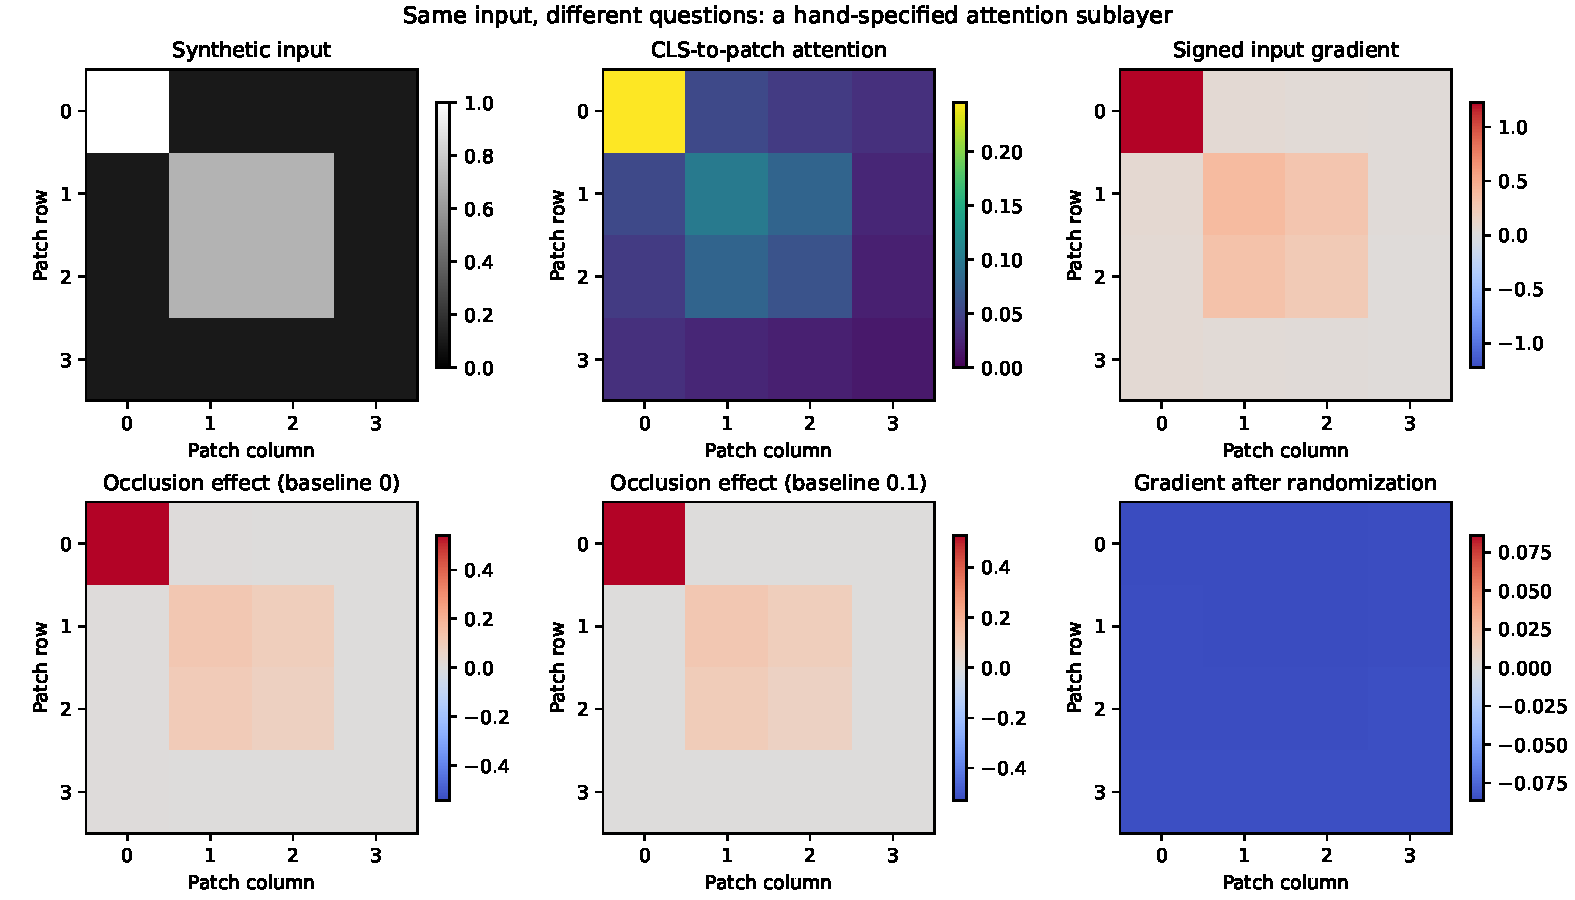
\includegraphics[width=\linewidth]{figures/attention_maps.pdf}
\caption{Computed maps from the same hand-specified self-attention sublayer. The central square is a synthetic pattern and the upper-left patch is a marker. Each panel has its own numerical scale: colours across panels are not directly comparable. The lower row compares two occlusion baselines and a gradient after parameter randomization. These are illustrative computational quantities, not anatomical explanations.}\label{fig:maps}
\end{figure}

For the supplied input, $f=1.586054$. Replacing the upper-left marker intensity 1.0 by the background value 0.1 leaves the central pattern unchanged and gives $f=1.057792$, a decrease of 0.528262. This demonstrates marker sensitivity by construction; it does not demonstrate that training learned a shortcut. In a second intervention, reversing the intensity contribution to the values leaves attention weights exactly unchanged but gives $f=-1.457165$. Thus the same attention display can accompany different outputs. Replacing all parameter arrays with seeded random draws supplies a further parameter-dependence illustration. Since no model is trained, this exercise does not implement a training-label randomization test and should not be presented as reproducing \citet{adebayo2018}.

The implementation computes the gradient analytically by the chain rule and verifies every input component against central finite differences with step $10^{-6}$. A central finite difference estimates a derivative by evaluating the output just above and below an input value and dividing the difference by twice the step. The maximum absolute discrepancy in the recorded check was below $10^{-8}$. It also checks row normalization and the unchanged attention matrix in the value-only intervention. The JSON output preserves full matrices, scores, both occlusion baselines, and package versions. After setting up the project environment as described in the repository, run the example from the project root:
\begin{verbatim}
python -m brainsmodels.attention_maps
\end{verbatim}
A notebook calls the same shared implementation in \path{code/notebooks/08_attention_maps.ipynb} with instructions. An extension for students is to change the occlusion baseline or readout while holding everything else fixed and predict which map will change. Applying these methods to a trained clinical system would additionally require a specified model, preprocessing, output target, valid intervention, and independent evaluation data.

\learningcheck{A weighted output depends on scores and values; a gradient and a finite replacement describe different changes to that output.}{If both scalar values equal $-3$, what output must any normalized pair of attention weights produce?}

\section{Hopfield memory: a cue, an update rule, and an energy}\label{app:hopfield}
\subsection{An explicit model of pattern completion}
A stored configuration can act as an attractor: nearby starting states may settle into it. A landscape analogy is helpful if used carefully. A state is a location, the energy is its height, and the update rule restricts the available moves. Descending does not guarantee arrival at the intended valley. The construction below specifies what ``descending'' means, making the analogy checkable rather than explanatory by itself.

Let $s\in\{-1,+1\}^{N}$ be the current state: a vector of $N$ units, each with sign $-1$ or $+1$. For a single target pattern $\xi$ of the same size, define
\begin{equation}
w_{ij}=\frac{\xi_i\xi_j}{N}\quad(i\ne j),\qquad w_{ii}=0,
\qquad E(s)=-\frac12\sum_{i,j}w_{ij}s_i s_j.
\end{equation}
The weights are symmetric. The zero diagonal excludes self-input, and the factor $1/2$ avoids counting each pair twice. This is a classical associative-memory construction motivated by \citet{hopfield1982}; the following calculations spell out the particular teaching example.

For a selected unit $i$, compute its local field $h_i=\sum_jw_{ij}s_j$, the weighted input from the other units. Set $s_i'=+1$ if $h_i>0$, $s_i'=-1$ if $h_i<0$, and retain $s_i$ if $h_i=0$. The prime marks the new value. All other units remain unchanged; this is an asynchronous update. Cycle through the units, repeating until a complete pass makes no changes. The plotting implementation uses two passes for its specified cue, which is sufficient for that example.

\subsection{Why this update cannot increase energy}
Only terms involving $i$ change. Symmetry and the zero diagonal give
\begin{equation}
\Delta E=E(s')-E(s)=-(s_i'-s_i)h_i.
\end{equation}
If the sign stays the same, $\Delta E=0$. If it changes, $s_i'=-s_i$ and $s_i h_i<0$, hence $\Delta E=2s_i h_i<0$. Our tie rule prevents changes at zero field. Thus every actual change strictly decreases energy. With a finite state space and repeated visits to every unit, this rule reaches a fixed point. It need not reach the global minimum or the desired pattern. Simultaneous updates change the argument and can produce cycles; the proof does not apply to arbitrary network dynamics.

\subsection{Connecting the proof to Figure~\ref{fig:hopfield}}
The target in the supplied code is
\[
\xi=(1,1,-1,-1,1,-1,1,-1,-1,1,1,-1).
\]
The cue flips units 1, 4, and 8 (indices 0, 3, and 7 in Python). Write $m=\sum_i\xi_i s_i$ for the unnormalized overlap. For this single-pattern construction,
\begin{equation}
E(s)=-\frac{m^2-N}{2N}.
\end{equation}
Initially $N=12$ and $m=6$, so $E=-1$. After the three incorrect signs are corrected, $m$ takes values 8, 10, and 12, giving energies approximately $-2.1667$, $-3.6667$, and $-5.5$. Updates of already aligned units leave the energy unchanged. These steps explain both the drops and flat segments in the plot.

For the first correction, unit 1 is misaligned with its target: $\xi_1=+1$ and $s_1=-1$. Its local field is $h_1=\xi_1(m-\xi_1s_1)/N=7/12$, so $s_1'=+1$. Substitution into the energy-change formula gives $\Delta E=-(1-(-1))(7/12)=-7/6$. Adding this to the starting energy $-1$ gives $-13/6\approx-2.1667$, matching the first drop in the recorded trajectory.

There is a revealing limitation even here: $-\xi$ has the same minimum energy as $\xi$ and is also stable. Energy minimization alone cannot distinguish the intended pattern from its inverse. With several patterns, one can use $w_{ij}=N^{-1}\sum_\mu\xi_i^\mu\xi_j^\mu$ for $i\ne j$, but interference and additional attractors complicate retrieval. A useful extension exercise is to vary the initial flips and stored patterns, recording which attractor is reached. The energy proof remains valid when its assumptions hold, while retrieval success can change. This separates a proved dynamical property from a claim about memory performance.

\learningcheck{The energy proof concerns an update rule under stated assumptions; retrieval success additionally depends on the cue and stored patterns.}{Why does starting at $-\xi$ give a counterexample to the claim that descending energy always recovers the intended target?}

\section{4E cognition: four questions about the clinical setting}\label{app:4e}
The 4E vocabulary identifies related but distinct emphases \citep{newen2018}. \emph{Embodied} approaches attend to bodily contributions to cognition. \emph{Embedded} approaches attend to its environmental and social setting. \emph{Enactive} approaches emphasize activity and ongoing organism--environment engagement. \emph{Extended} approaches ask whether some external resources can be constituents of cognition. The distinction between a causal influence and a constituent is consequential: showing that a tool changes performance is insufficient, by itself, to establish that it is part of a mind.

The following applications are proposed teaching examples, rather than empirical findings about radiology teams.

\begin{table}[htbp]\centering\small
\caption{Applying the four questions to the hypothetical MRI review. The examples translate concepts into investigable workflow questions.}
\begin{tabularx}{\linewidth}{p{21mm}XX}\toprule
Emphasis & Illustrative question & A possible comparison \\\midrule
Embodied & Does the clinician's bodily state affect sustained inspection and interpretation? & Compare controlled viewing tasks across recorded fatigue or ergonomic conditions.\\
Embedded & How does access to prior scans, team discussion, and the reporting environment shape interpretation? & Compare available information and coordination under specified workflows.\\
Enactive & How does scrolling, changing the view, and revisiting a region alter the evidence obtained? & Compare active image exploration with matched prerecorded viewing.\\
Extended & Does a reliably integrated record function as part of the ongoing reasoning process? & Document patterns of reliance and disruption, while separating performance effects from the constitutive claim.\\\bottomrule
\end{tabularx}
\end{table}

Under suitable functional integration, the extended-mind proposal treats external resources as constituents of a cognitive process \citep{clark1998}. A performance difference with and without a longitudinal record measures dependence on the record; identifying it as a cognitive constituent requires an additional argument.

Specify what each comparison holds constant. Prerecorded viewing can change both agency and visual evidence; withdrawing a record changes task difficulty as well as tool availability. These alternatives need controls, as in the earlier shortcut example.

The four questions broaden the explanation of a clinical decision to include the patient, clinician, tool and environment, each with a proposed observable role.

\learningcheck{A workflow study can measure dependence on a tool while leaving the stronger claim about cognitive constitution open.}{If withdrawing a longitudinal record reduces accuracy, which task-difficulty explanation would you need to examine before making an extended-mind claim?}
